%%This is a very basic article template.
%%There is just one section and two subsections.
\documentclass[12pt,  a4paper]{scrartcl}
\usepackage[latin1]{inputenc}
\usepackage[T1]{fontenc}
\usepackage{graphicx}
\usepackage{epstopdf}
\usepackage{avant}
\usepackage[ngerman]{babel}
\usepackage[a4paper, top=3cm, bottom=3cm, left=2.5cm,
right=1.5cm]{geometry}
\usepackage{fancyhdr}
\usepackage{listings}
\usepackage{paralist}
\usepackage{color}


\definecolor{darkblue}{rgb}{0,0,.5}
\usepackage{hyperref}
\hypersetup{colorlinks=true, breaklinks=true, linkcolor=darkblue,
menucolor=darkblue, urlcolor=darkblue}
\usepackage{breakurl}

\usepackage{url}

\usepackage[cc]{titlepic}
\usepackage{graphicx}
\titlepic{
\includegraphics{images/Xtext-logo-dark.eps}}


\usepackage{tabularx}

\addtokomafont{sectioning}{\color{darkblue}}
\addtokomafont{subsubsection}{\color{darkblue}}

\usepackage{lmodern}


% Setzen des Headers
\setlength{\headwidth}{\textwidth}
\fancyhead[L]{\raisebox{-0.05cm}{
\includegraphics[height=0.6cm]{images/itemis_logo_4c.eps}}}
\fancyhead[R]{\fontfamily{pag}\selectfont{\textbf{LWC13 -
\raisebox{-0.09cm}{
\includegraphics[height=0.5cm]{images/Xtext-logo-dark.eps}} Submission}}}

% Wir wollen eine "Fancy" Ausgabe
\pagestyle{fancy}

% Absatzformatierung
\frenchspacing
\parindent 0pt      % kein Einrcken bei neuem Absatz
\parskip 10pt    	% Abstand zwischen den Absaetzen

% Listingsformatierung
\lstloadlanguages{Java, XML}
\lstset{
    language=Java,
    showspaces=false,
    showstringspaces=false,
    basicstyle=\small\ttfamily\footnotesize,
    columns=fullflexible,% typewriter font look better with fullflex
    keywordstyle=\color[rgb]{0.627,0.165,0.467},
    stringstyle=\color[rgb]{0.286,0.172,0.980},
    commentstyle=\color[rgb]{0.294,0.565,0.478},
    tabsize=2,
    numbers=left,
    numberstyle=\scriptsize,
    breaklines=true,
    identifierstyle=\ttfamily,
    backgroundcolor=\color[rgb]{0.9, 0.9, 0.9},
    rulesepcolor=\color[rgb]{0.3, 0.3, 0.3},
    captionpos=b,
    frame=shadowbox,
    otherkeywords={@SuppressWarnings,@Singleton,@Check,@Inject}
}
\lstdefinelanguage {Xtext}[]{Java} {
    morekeywords={returns,generate,as,import,with,grammar}
}
\lstdefinelanguage {Xtend}[]{Java} {
    morekeywords={def,dispatch,override,val,IF,ENDIF,FOR,ENDFOR,typeof,@Inject,extension}
%    otherkeywords={+=,=,\{,\}}
}
\lstdefinelanguage {Mwe2}[]{Java} {
    morekeywords={module,var,component,bean}
}
\lstdefinelanguage {dmodel}[]{Java} {
    morekeywords={datatype,entity,op,\:}
}
\lstdefinelanguage {instances}[]{Java} {
    morekeywords={\=}
}

%
%%% Trennungsregeln fuer das gesamte Dokument.
%
\hyphenation{language-work-benches domain-model
Generate-Domain-model-Language}

\renewcommand{\baselinestretch}{1.25}

\begin{document}
\begin{titlepage}

\begin{center}

% Upper part of the page
\raisebox{-6cm}{
  
\includegraphics[width=10cm]{./images/Xtext-logo-dark.eps}
}
\\[3cm]


% Title
\rule{\linewidth}{0.7mm}
\\[0.4cm]


    \fontfamily{pag}\selectfont
    \LARGE{\color{darkblue}Language Workbench Challenge 2013 \\
    Xtext Submission} \\[0.5cm]

    \color{black}
    \large{Version: 1.0 - DRAFT \today}
%    \large{Version: 1.1 DRAFT - \today}
    \\[0.4cm]
\rule{\linewidth}{0.7mm}
\\[1.5cm]
\normalfont

% Author
\fontfamily{pag}\selectfont
Karsten Thoms, Johannes Dicks, Thomas Kutz (itemis)
\normalfont

\vfill

% Bottom of the page
%{\large \today}

\end{center}

\end{titlepage}  


\newpage

\section*{Abstract}
The Language Workbench Competition 2011 (LWC11) is an initiative created by a
group of experts at the CodeGeneration 2010
conference\footnote{\url{http://www.codegeneration.net/cg2010/}}. The aim is to
set a common task\footnote{see \url{http://www.languageworkbenches.net/} for the
detailed description of the LWC11 competition and other submissions}
for Language Workbenches\footnote{\url{http://martinfowler.com/articles/languageWorkbench.html},
\url{http://blog.efftinge.de/2007/11/definition-of-term-language-workbench.html}}
which is implemented with the different existing alternatives in a comparable
way. This document describes in detail how the task is solved with
Xtext\footnote{\url{http://www.xtext.org}}. Xtext is one of the most well known
Language Workbenches and part of the Eclipse Modeling
Project\footnote{\url{http://www.eclipse.org/modeling}}.


\section*{Testimonial}
This project was developed with the help of some colleagues at itemis, and I am
grateful for their help:

\begin{compactenum}
  \item \emph{Sven Efftinge} contributed the Instance DSL. Without his knowledge
  it would be very hard to implement this project already with Xtext 2.0 in this
  pre-release state.
  \item \emph{Rainer Klute} has written the initial version of the introduction.
  Although at that time the task was realized with Xtext 1.0.2 and many places
  have been reworked, major parts of the Overview and Phase 0.1 descriptions are
  based on his contribution.
  \item \emph{Karsten Nolte and Alexander Hannweg} initially transformed the
  Wiki pages to LaTeX.
  \item \emph{The Xtext Development Team} was always responsive for questions
  , provided with the Domainmodel example a good template to create major parts
  of the implementation and was eager to fix detected bugs.
  \item Detailed feedback helped to improve the document. My thanks for
  reading the document carefully and providing input go to
  \footnote{Not all from itemis}
  : \emph{Markus V�lter, J�rg Reichert, Joel W. Denton}
\end{compactenum}

\newpage
\section*{Document History}

\textbf {Version 0.1 - 2013-01-28}
\begin{compactitem}
\item Initial creation \\
\end{compactitem}

\textbf {Version 1.0 - 2013-04-08}
\begin{compactitem}
\item Final version for the Language Workbench Challenge workshop in Cambridge
\\
\end{compactitem}


\newpage

\renewcommand{\contentsname}{Table Of Contents}
\tableofcontents

\newpage

\normalsize

\section{Introduction}

\subsection{Task Description}
The {\href{http://www.languageworkbenches.net/images/5/53/Ql.pdf}{LWC13 task}}
is to implement a DSL for questionnaires (Questionnaire Language, QL), which
basically allows the definition of forms with questions.


\subsection{Technology Stack}
This tutorial expects that you are somehow familiar with Java and Eclipse and
have heard about \url{EMF} and how it works in general before. We start almost at the
beginning, but not quite :-) 

We will use Xtext 2.3.1, which is at the moment of writing the latest official
release.
Xtext 2.4 is in preparation and will be released with Eclipse Kepler in June
2013\footnote{\url{http://wiki.eclipse.org/Kepler/Simultaneous_Release_Plan}}.
The solution approach described here would work also with any version
of Xtext >= 2.0, but the API might differ slightly, so there is no guarantee
that each codeline printed here would work exactly with all versions. For better
reproduction it is highly recommended to use the versions mentioned above.

For Code Generation we will use the language Xtend, which itself is based on
Xtext. Xtend makes use of a common expression language shipped with Xtext called
Xbase. The languages developed here will also be based on Xbase, but more on
this later.

The reference implementation of the Xtend generator will generate, 
JavaServer Faces 2.1( JSF).\footnote{\url{http://www.javaserverfaces.org/}} 
JSF is part of the Java Enterprise Edition (Java EE). It is useful to have a 
basic understanding of how web applications work even if JSF provides a nice level 
of abstraction. The JSF reference implementation from 
Oracle Mojarra 2.1.6\footnote{\url{http://javaserverfaces.java.net/}} is able to run 
within the well known Servlet container Apache Tomcat( v7.0).\footnote{\url{http://tomcat.apache.org/}} 

To get a nicely integrated developement environment we will install some components of the
Web Tools Platform( WTP)\footnote{\url{http://www.eclipse.org/webtools/}} into an existing Eclipse installation.
\subsection{Installing Eclipse and Xtext}

Xtext is a SDK for the \href{http://www.eclipse.org/}{Eclipse} IDE. To
install it you have two options:

\begin{compactitem}
    \item You can download Xtext separately and install it in your Eclipse
    instance.
    \item You can download a specially-crafted complete Eclipse distribution
    which has Xtext prepackaged already.
\end{compactitem}

We will take the latter approach here and describe the individual steps:

\begin{compactenum}
    \item Go to the \href{http://xtext.itemis.com/xtext/language=en/36553/downloads/}{Xtext download
    page}. Here you can get Eclipse 4.2.x (Juno) including Xtext 2.3.1
    along with some tools Xtext depends on. The latter are subsumed here under
    ``Xtext'' for simplicity.
    If you want you can download also a distribution
    which is already bundled with Eclipse 4.3.0 Kepler, but be aware that this
    is not finalized until end of June 2013.
    \item The Eclipse/Xtext distribution is available for multiple platforms.

    \begin{compactenum}
      \item
      \href{http://download.itemis.com/distros/eclipse-SDK-4.2-Xtext-2.3.1-linux-gtk-x86_64.tar.gz}{Linux GTK x86 64 bit}
      \item
      \href{http://download.itemis.com/distros/eclipse-SDK-4.2-Xtext-2.3.1-linux-gtk.tar.gz}{Linux GTK x86 32 bit}
        \item
        \href{http://download.itemis.com/distros/eclipse-SDK-4.2-Xtext-2.3.1-macosx-cocoa-x86_64.tar.gz}{Mac OSX x86 64 bit}
        \item
        \href{http://download.itemis.com/distros/eclipse-SDK-4.2-Xtext-2.3.1-win32-x86_64.zip}{Windows 64 bit}
        \item
        \href{http://download.itemis.com/distros/eclipse-SDK-4.2-Xtext-2.3.1-win32.zip}{Windows 32 bit}
    \end{compactenum}

    \item Unpack the downloaded archive file in a directory of your choice.

        Example (Linux):

\begin{lstlisting}
  cd /opt/local
  gzip -dc /download/eclipse-SDK-4.2-Xtext-2.3.1-linux-gtk-x86_64.tar.gz | tar
  xvfp -
\end{lstlisting}

        The archive will be extracted to a new directory named \texttt{eclipse}. Before
        unpacking the archive, please ensure that there is no subdirectory named
        \texttt{eclipse} yet! Different operating systems may require different unpacking
        methods.\footnote{On Windows do not unpack it into a deep directory,
        since this might cause troubles with long path names.}

    \item Start Eclipse by running the \texttt{eclipse} executable in the newly-created
    \texttt{eclipse} directory.
\end{compactenum}

\subsection{Workspace Setup}

Before we begin, start Eclipse and set up a fresh workspace.

Some settings should be done. Open the workspace settings:

\begin{compactitem}
    \item Windows: Window / Preferences
    \item Mac: Eclipse / Preferences
\end{compactitem}

\paragraph{Workspace Encoding}
$\;$ \\
File encoding is important to some type of files. It is better that the
workspace is set to a common encoding to avoid any platform specific encoding.
By default the workspace is using platform encoding, which is Cp1252 on Windows
and MacRoman on Mac. We will use ISO-8859-1 as a common encoding here.

\begin{compactitem}
    \item Open Eclipse Preferences and go to \emph{General / Workspace}
    \item Change setting \emph{Text file encoding} to \emph{Other /
    ISO-8859-1}
\end{compactitem}

\paragraph{Launch Operation}
$\;$ \\

\begin{compactitem}
    \item Open Run/Debug / Launching
    \item Change ``Launch Operation'' to ``Always
    launch the previously launched application''
\end{compactitem}
This will allow you re-running the previous launched application by just
pressing the Run or Debug button in the Eclipse toolbar, or using keyboard
shortcuts. The default settings does not always do what you want.



\section{Developing the Questionnaire Language}

\section{Developing the Questionnaire Language}

Step 1: Set up initial language implementation
- Create Project
- Define Grammar
- Generate Implementation

\subsection{Generate Language Implementation}

Now that the initial grammar of the language has been defined it is time to test
the language. Xtext ships with a code generator which generates all the glue
code needed for the language implementation.

To generate the code, we need to execute the generator workflow
\texttt{GenerateQlDsl.mwe2}. For this, select the workflow file, open the context menu
and select \emph{Run As / MWE2 Workflow}.

The generator will print some information to the Console, and finally it should
print \texttt{``Done.''}.

\begin{lstlisting}
0    [main] INFO  lipse.emf.mwe.utils.StandaloneSetup  - Registering platform
uri ....
   ...
13727 [main] INFO  .emf.mwe2.runtime.workflow.Workflow  - Done.
\end{lstlisting}

After successful execution the projects will be filled with implementation code.
Code that will be regenerated each time the generator is executed will go to the
source folder \texttt{/src-gen} (in all three projects), whereas code generated to
\texttt{/src} will be generated only once as skeleton. It is safe to edit these
classes.

Xtext follows the Generation Gap
Pattern\footnote{\url{http://heikobehrens.net/2009/04/23/generation-gap-pattern/}}:
Generated code is based on the Xtext API. Manual code is separated from
generated code. Often manual classes are derived from generated classes to allow
overriding of generated code or adding functionality.

Investigate the generated code a bit. Some pieces to mention:
\paragraph{Runtime Project - folder \texttt{src}}
\begin{itemize}
\item The class \texttt{QlDslRuntimeModule} is a Guice configuration.
Guice\footnote{\url{http://code.google.com/p/google-guice/}} is a famous
Dependency Injection\footnote{\url{http://en.wikipedia.org/wiki/Dependency_injection}} framework in Java. 
Xtext makes heavy use of Dependency Injection, which in turn allows to exchange
nearly every bit of the framework for customizing or to work around limitations,
if necessary, without the need to change the framework itself.
\item Class \texttt{QlDslStandaloneSetup} is needed when using the language in
``standalone mode'', i.e. without an Eclipse environment. Eclipse plugins, like
Xtext and the language plugin, usually need an OSGi container as execution
environment. Xtext is designed to be executable without the need to be
deployed into an OSGi container, but for this certain registrations are
required which an OSGi container would usually provide automatically. This is
especially useful when Xtext based languages are used in build environments or
other IDEs.
\item Class \texttt{QlDslFormatter} allows the implementation of a declarative
code formatter for the DSL.
\item File \texttt{QlDslJvmModelInferrer.xtend} is a class implemented with the
Xtend language. The JVM Model Inferrer will play an important role later when we
introduce expressions and code generation.
\item Class QlDslJavaValidation allows the implementation of validation rules
for the DSL.
\end{itemize}


\paragraph{Runtime Project - folder \texttt{src-gen}}
\begin{itemize}
  \item The Ecore metamodel is generated to file \texttt{QlDsl.ecore}.

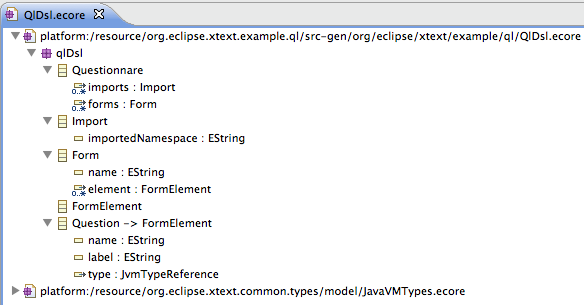
\includegraphics[width=16cm]{./images/chapter01/QlDsl_ecore.png}

  \item The Java implementation code for the metamodel can be found in the
  package \newline\texttt{org.eclipse.xtext.example.ql.qlDsl}.
  \item The package \texttt{org.eclipse.xtext.example.ql.parser.antlr.internal}
  contains an \newline ANTLR3\footnote{\url{http://www.antlr.org}} grammar and
  the Lexer and Parser classes generated from it.
\end{itemize}


\section{Testing the Questionnaire Language}

\subsection{Creating a Launch Configuration}

In order to test the language and the editor we need to deploy the developed
plugins within another Eclipse instance. For testing the easiest way is start a
so-called Runtime Instance.

Open the dialog \emph{Run / Run Configurations} and select the node \emph{Eclipse
Application} from the left tree widget and press the icon with the +
sign to create a new Launch Config.

You could leave the defaults here or change the name and location like in the
screenshot.

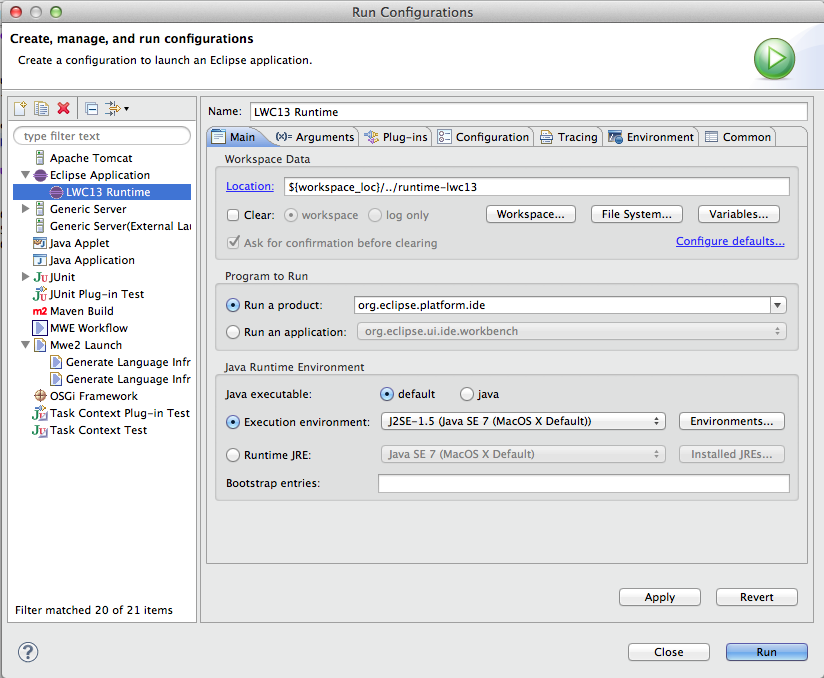
\includegraphics[width=17cm]{./images/chapter01/LaunchConfig.png}

Now switch to the Arguments page and enter in the ``VM arguments'' text box:
\begin{lstlisting}
-Xms40m -Xmx512m -XX:MaxPermSize=150m
\end{lstlisting}
Especially important is the MaxPermSize setting, since the default size of the
PermGen space of the VM (64MB) often is not enough.

Now press the \emph{``Run''} button. Another Eclipse instance will start with an
empty workspace. Close the Welcome window.


\subsection{Create Test Project}

In the Runtime Workspace create a new Java Project with name ``QLTest''.

Select the \texttt{/src} folder and create a new file
\texttt{``housepurchase.ql''}. Once you have created the file a popup dialog
will appear to ask, if you would like to add the Xtext nature on this project.
Answer with ``Yes''.

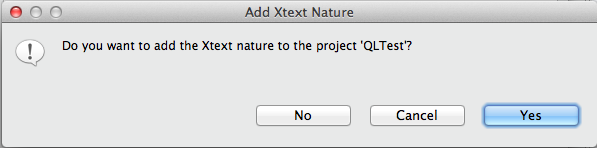
\includegraphics[width=12cm]{./images/chapter01/AddXtextNature.png}

From now on your project will be considered to contain files that Xtext should
recognize (\texttt{.ql} files). Projects having the Xtext nature will be processed by the
Xtext Builder when building projects, other projects are ignored. The Xtext
Builder indexes the Xtext based resources, links the cross-references in the
editor, and validates the model files. On errors, resource markers are created
which can be seen in the editor and the \emph{Problems View}.


\subsection{Xbase}

The language developed in section \ref{sec:DefiningGrammar} does not yet meet all 
demands on the LWC2013 task. Two core features are missing: First, a question's 
answer can be computed, i.e. its answer can be derived from an expression referring 
to previous questions' answers. Second, questions can be optional depending on the 
previous answers. For this, also the possibility to define expressions is needed. This
is where Xbase comes into play.

Xbase is an expression language which can be reused in your own Xtext DSL. Its language
concepts are similar to Java, but with some syntactical derivations improving readability.
The Xbase grammar is defined in Xtext, thus its elements can be used in any other Xtext grammar
by importing or directly extending Xbase via Xtext's possibility for grammar inheritance.
In addition to the grammar, Xbase ships with further infrastructural parts like a compiler, 
interpreter, linker or static analyzer which all can be adapted to your own needs. In
the background, Xbase produces plain Java code which is run on the JVM. Like
other DSLs defined with Xtext, Xbase provides also editor features like syntax highlighting, 
content assistance and navigation via hyperlinks. In the following we will first introduce
some language concepts of Xbase, and afterwards we will describe how to integrate Xbase
into the Questionnaire DSL.

In Xbase everything is an expression which always has a return type which might be \texttt{null} 
for some expressions. Variables are defined with the \texttt{var} keyword, whereas for 
constant values the \texttt{val} keyword is used. Types are derived automatically, so they 
don't need to be defined explicitly:

\begin{lstlisting}[language=Xbase]
var myVariable = 'some modifiable value'
val Integer myConstant = 42  
\end{lstlisting}

Xbase ships with a library extending existing Java types like String or Integer with further 
functionality. So besides the already known String operations from Java like 
\texttt{toUpperCase} or \texttt{toLowerCase}, in Xbase expressions you can also use \texttt{toFirstUpper}
and \texttt{toFirstLower} changing only the first letter's case which might come in handy 
in some situations. Large numbers can be written more readable by using underscores to
separate digits:

\begin{lstlisting}[language=Xbase]
"a day has ".toFirstUpper() + 86_400_000 + " milliseconds."
// results in: A day has 86400000 milliseconds.
\end{lstlisting}

As in Java, Xbase provides \texttt{if-else}-expressions for defining conditions. Since each expression
has a return type, it is valid to use  \texttt{if-else}-blocks similar to the ternary operator in Java:

\begin{lstlisting}[language=Xbase]
var x = if (condition) 42 else 43
\end{lstlisting}

There are further concepts in Xbase which we will not cover here in more detail, since they have
not much relevance for the questionnaire language. So e.g. it is possible to use loops for
iterating over a collection of element; there is a \texttt{switch-case}-expression
with type guards allowing for defining behavior depending on the type of a parameter; and last but
not least, Xbase allows the definition of closures. For more details, please look up the reference
documentation\footnote{\url{http://www.eclipse.org/Xtext/documentation.html#xbaseLanguageRef_Introduction}}
or the Xbase tutorials directly in Eclipse (\emph{File / New / Other.. / Xbase Tutorial}). 

With these capabilities integrated in the Questionnaire language it is feasible to define complex
domain logic e.g. for the result of a questionnaire directly in its definition. For example, when
designing a questionnaire for a test, let's say to define a person's stress level, you can write
some Xbase code as expression for the last ``result'' question:

\begin{lstlisting}[language=Xbase]
stressLevelResult: "Your Stress-Level: " String (
	{
		var Integer stressPoints = if (hasTimePressureAtWork) 30 else 0
		stressPoints = stressPoints + daysSleepingBadPerWeek * 3
		stressPoints = stressPoints + glassesOfAlcoholPerDay * 12
		stressPoints = stressPoints - daysWithSportPerWeek * 2
		if (stressPoints>80) "High" else if (stressPoints>40) "Medium" else "Low"
	}
) 
\end{lstlisting}

\section{Including Expressions into the QL Language}

- Derive Grammar from Xbase
- Generate Implementation

\subsection{JVM Model Inference}

For languages using Xbase it is necessary to tell Xtext, how to map concepts of a language to a Java model. In our example,
a Form could be mapped to the Type concept, while Questions are the fields of a class. By doing this, elements of the language
can be made available in expressions. Further, it allows that model elements are linkable where Java types are expected, without
necessarily generate a Java class.

The derivation of the Java model for language concepts is the responsibility of the JVM Model Inferrer, which is a class that implements
the \href{http://download.eclipse.org/modeling/tmf/xtext/javadoc/2.3/org/eclipse/xtext/xbase/jvmmodel/IJvmModelInferrer.html}{\texttt{IJvmModelInferrer}} interface.
A skeleton has already been generated into package \texttt{org.eclipse.xtext.example.ql.jvmmodel}. The file \texttt{QlDslJvmModelInferrer.xtend} is a class
written with Xtend.

The mapping that has to be implemented for the Questionnaire DSL should be as follows:
\begin{enumerate}
  \item Each \texttt{Form} instance is mapped to a \texttt{JvmDeclaredType} (which is the common concept for Java classes and interfaces).
  The type's name is simply the form name, and the target package is forms.
  \item Each \texttt{Question} of a \texttt{Form} is mapped to a \texttt{JvmField}, which is added as member of the declared type
  \item For each \texttt{Question} accessor methods for the field are generated. The field gets only a setter if the value of the Question is
  not computed by an expression. If the field is computed, the content of the getter has to compute the result.
  \item For each \texttt{Question} a method \texttt{is<QUESTIONNAME>Enabled()} is inferred.
  Questions with computed values are not enabled.
  \item For each \texttt{ConditionalQuestionGroup} a method is produced that computes
  whether the group is visible or not. 
\end{enumerate}

Now place the content into the inferrer class\footnote{\url{https://gist.github.com/kthoms/5132153}}
: 
\begin{lstlisting}[language=Xtend]
package org.eclipse.xtext.example.ql.jvmmodel

import com.google.inject.Inject
import java.io.Serializable
import org.eclipse.xtext.common.types.JvmOperation
import org.eclipse.xtext.common.types.util.TypeReferences
import org.eclipse.xtext.example.ql.qlDsl.ConditionalQuestionGroup
import org.eclipse.xtext.example.ql.qlDsl.Question
import org.eclipse.xtext.example.ql.qlDsl.Questionnaire
import org.eclipse.xtext.xbase.XExpression
import org.eclipse.xtext.xbase.XbaseFactory
import org.eclipse.xtext.xbase.jvmmodel.AbstractModelInferrer
import org.eclipse.xtext.xbase.jvmmodel.IJvmDeclaredTypeAcceptor
import org.eclipse.xtext.xbase.jvmmodel.JvmTypesBuilder

class QlDslJvmModelInferrer extends AbstractModelInferrer {
  @Inject extension JvmTypesBuilder
  @Inject TypeReferences typeReferences

def dispatch void infer(Questionnaire element, IJvmDeclaredTypeAcceptor acceptor, boolean isPreIndexingPhase) {
    for (form: element.forms) {
      acceptor.accept(form.toClass("forms."+form.name))
      .initializeLater[
        //implements Serializable
        it.superTypes +=typeReferences.getTypeForName(typeof(Serializable),element,null)

        members += toField("serialVersionUID",typeReferences.getTypeForName("long",element),[final = true ^static = true 
          setInitializer([it.append("1L")])
        ])

        val allQuestions = form.eAllContents.filter(typeof(Question)).toList
        
        for (question: allQuestions) {
          members += question.toField(question.name, question.type)
        }

        for (question: allQuestions) {
          if (question.expression == null) {
            members += question.toGetter(question.name, question.type)
            members += question.toSetter(question.name, question.type)
          } else {
            val getter = question.toGetter(question.name, question.type)
            getter.body = question.expression
            members += getter
          }
          members += question.createIsEnabledMethod
        }

        val allQuestionGroups = form.eAllContents.filter(typeof(ConditionalQuestionGroup)).toList
        var groupIndex=0;
        for (questionGroup: allQuestionGroups) {
          members += questionGroup.createIsGroupVisibleMethod(groupIndex)
          groupIndex = groupIndex+1
        }

      ]
    }
  }

   def JvmOperation createIsEnabledMethod (Question question) {
     question.toMethod("is"+question.name.toFirstUpper+"Enabled", typeReferences.getTypeForName("boolean", question, null)) [
       body = [it.append('''return «question.expression == null»;''')]
    ]
   }

   /** Create a method <code>public boolean isGroup[groupIndex]Visible ()</code>.*/
   def JvmOperation createIsGroupVisibleMethod (ConditionalQuestionGroup group, int groupIndex) {
     group.toMethod("isGroup"+groupIndex+"Visible", typeReferences.getTypeForName("boolean", group, null)) [
       if(group.condition != null) {
         body = group.condition
       } else {
         body = [it.append('''return true;''')]
       }
     ]
   }

}
\end{lstlisting}

Now lets take a deeper look at the implementation:

\begin{lstlisting}[language=Xtend]
class QlDslJvmModelInferrer extends AbstractModelInferrer {
  @Inject extension JvmTypesBuilder
  @Inject TypeReferences typeReferences
  def dispatch void infer(Questionnaire element, IJvmDeclaredTypeAcceptor acceptor, boolean isPreIndexingPhase) {
     ...
  }
}
\end{lstlisting}

The inferrer class implements \texttt{IJvmModelInferrer}, but for convenience we derive
from its abstract implementation \texttt{AbstractModelInferrer}. The main method to
implement is \texttt{infer()}. In the case of QL models, the root element
of model resources is a \texttt{Questionnaire}. The base implementation uses polymorphic dispatching on
the root element of a model resource, and the \texttt{infer()} method of our
implementation hooks into the dispatching by using the dispatch keyword. That is
also why the first argument can be of type \texttt{Questionnaire}, and not of the base
type \texttt{EObject}, like defined in the \texttt{infer()} method that is definied in
\texttt{IJvmModelInferrer}.

The implementation uses two services, which are injected as members into the
class:
\begin{itemize}
\item The \texttt{JvmTypesBuilder} offers factory and builder functions to create
instances of JVM Model types. The additional keyword \texttt{extension} has the effect,
that the methods of the \texttt{JvmTypesBuilder} become so-called \textbf{extension methods}.
This means, the functions become implicitly available as additional
methods on the first argument of the function. We will see extensive use of this
nice feature of Xtend in the implementation of the Xtend based code generator in
the next chapter.
\item \texttt{TypeReferences} is used to retrieve the respective JVM Model instances for
given qualified Java class names through its \texttt{getTypeForName()} methods. 
\end{itemize}

\begin{lstlisting}[language=Xtend]
    for (form: element.forms) {
      acceptor.accept(form.toClass("forms."+form.name))
      .initializeLater[
         ...
      ]
    }
\end{lstlisting}

Let's take a deeper look on the \texttt{infer()} method. The outer loop simply
iterates over the \texttt{Form} instances of the \texttt{Questionnaire} element.
Inside the loop we first derive a Class instance for each \texttt{Questionnaire}
element in package \texttt{forms}. JVM Model Inference is executed in two
phases: In the first phase all types are derived, without any content. In the
second phase, the content of the types is derived. This is done by the closure
passed to \texttt{initializeLater()}. The reason why this has to happen this way
is that during inference of type members, they could refer again to types that
are derived by the inferrer. The two phases prevent circular calls.

\begin{lstlisting}[language=Xtend]
it.superTypes +=typeReferences.getTypeForName(typeof(Serializable),element,null)

members += toField("serialVersionUID",typeReferences.getTypeForName("long",element),
[final = true ^static = true 
  setInitializer([it.append("1L")])
])
\end{lstlisting}
        
We want to make the resulting Java class serializable. This is optional, but
better style. Therefore the class has to implement the \texttt{java.io.Serializable}
interface, whose JVM Model representative is retrieved from the \texttt{TypeReferences}
instance and added to the \texttt{superTypes} collection. The identifier \texttt{it} denotes the
implicit variable of type Form of the closure. It is not necessary to qualify it
here, it could be left out. The closure passed to the \texttt{setInitializer()}
method initializes the field with the value ``1'' of type long.

\begin{lstlisting}[language=Xtend]
val allQuestions = form.eAllContents.filter(typeof(Question)).toList

for (question: allQuestions) {
  members += question.toField(question.name, question.type)
}
\end{lstlisting}

All \texttt{Question} instances from the resource are bound to the final variable
\texttt{allQuestions}. Since Questions can be nested into groups, the content has to be
searched recursively. \texttt{eAllContents} will traverse over all elements.

Next, for each \texttt{Question} a \texttt{JvmField} instance is inferred. Here the
\texttt{JvmTypesBuilder} is helping us with the method \texttt{toField}, which gets the name and
type of the derived field. Here we see the effect of the extension keyword: It
seems that \texttt{toField} is actually a method of type Question, but it is a method of
the \texttt{JvmTypesBuilder} class.

\begin{lstlisting}[language=Xtend]
for (question: allQuestions) {
  if (question.expression == null) {
    members += question.toGetter(question.name, question.type)
    members += question.toSetter(question.name, question.type)
  } else {
    val getter = question.toGetter(question.name, question.type)
    getter.body = question.expression
    members += getter
  }
  ...
}
\end{lstlisting}

The next loop creates the accessor methods for the fields. We could have done
this in the previous loop also, but it is better style to declare the fields
first, and methods next in the class. The inferred \texttt{JvmDeclaredType} will be
translated to Java later, so it is better to have that clean from the beginning.

Within the loop, we decide if the question has a computation expression or not.
If it hasn't one, it is a simple field with getter and setter, where we call the
\texttt{toGetter()}/\texttt{toSetter()} builder functions. If the question value is computed by an
expression, it does not make sense to offer a setter method. The field needs to
be read-only. The getter method does not simply return the value of a field.
Instead, the method has to evaluate the expression. Thus, we assign the
expression as body of the method.

\begin{lstlisting}[language=Xtend]
for (question: allQuestions) {
  ...
  members += question.createIsEnabledMethod
}

...
def JvmOperation createIsEnabledMethod (Question question) {
  question.toMethod("is"+question.name.toFirstUpper+"Enabled",
 typeReferences.getTypeForName("boolean", question, null)) [ body = [it.append('''return «question.expression == null»;''')]
  ]
}
\end{lstlisting}

For each \texttt{Question} a method \texttt{boolean is<QUESTIONNAME>Enabled()}
is inferred. The body of the method does simply return \texttt{true} if the Question does
not have an computation expression assigned, or \texttt{false} otherwise.

In this case we assign to the body a closure that computes the method
implementation text. This is the first example where we make use of Xtend's \emph{Rich
String} feature (the text between the three single quotes '''), which is
later heavily used in the code generator templates.

\begin{lstlisting}[language=Xtend]
val allQuestionGroups = form.eAllContents.filter(typeof(ConditionalQuestionGroup)).toList
var groupIndex=0;
for (questionGroup: allQuestionGroups) {
  members += questionGroup.createIsGroupVisibleMethod(groupIndex)
  groupIndex = groupIndex+1
}

def JvmOperation createIsGroupVisibleMethod (ConditionalQuestionGroup group, int groupIndex) {
 group.toMethod("isGroup"+groupIndex+"Visible", typeReferences.getTypeForName("boolean", group, null)) [
   if(group.condition != null) {
     body = group.condition
   } else {
     body = [it.append('''return true;''')]
   }
 ]
}
\end{lstlisting}

We now filter all \texttt{ConditionalQuestionGroup} instances from the \texttt{Questionnaire} and
loop over them. For each of them, a method \texttt{is<QUESTIONGROUPINDEX>Visible()} 
is produced. Unfortunately, question groups are anonymous, thus we
maintain an index counter and name the methods \texttt{isGroup<IDX>Visible()}.

Since condition expressions for groups are optional, the method body has to
return simply \texttt{true} in the case that no expression is assigned. When groups have
a condition, the condition expression is assigned as the method body.





\end{document}